\documentclass{beamer}
\usepackage{lmodern}  % text format combination, bold+it
\usetheme[progressbar=frametitle]{metropolis}
\setbeamertemplate{frame numbering}[fraction]
\useoutertheme{metropolis}
\useinnertheme{metropolis}
\usefonttheme{metropolis}
\usecolortheme{spruce}
\setbeamercolor{background canvas}{bg=white}
\usepackage{multicol}
\usepackage{amsmath}  %math staff
\usepackage{graphicx}  %import images
\usepackage{float} %control float positions
\usepackage{amsbsy}
\title{Simulation Report 1}
\author{Jinxi Liu}
\begin{document}
	\metroset{block=fill}
	
\begin{frame}
	
	\titlepage
	
\end{frame}


\begin{frame}[t]{Introduction}\vspace{10pt}
Suppose we have $z_i \sim N(0,1)$, $i=1,2$ under the null. Their correlation is $\rho$. We perform a one-sided test with rejection region $\Gamma = \{z \geq 1.645\}.$

We then estimate $FDR(\Gamma)$ by 
\begin{equation}\label{eq1}
 \hat{FDR}(\Gamma) = \frac{\hat{\pi}_0 E[R^0(\Gamma)]}{ R(\Gamma)\vee 1}
\end{equation}
Since we have only two variables and $R(\Gamma)\vee 1$ is observable, we only focus on the numerator of equation(\ref{eq1}).
\end{frame}

\begin{frame}[t]{Theoretical derivation}\vspace{10pt}
\begin{equation} \label{eq2}
\begin{split}
E[R^0(\Gamma)]  &= P\{R^0(\Gamma) =1 \} \times 1 + P\{R^0(\Gamma) =2 \} \times 2 \\
 &= p\{z_1 > 1.645 \ and \ z_2 \leq 1.645 \ or \ z_2 > 1.645 \ and \ z_1 \leq 1.645 \} \\
 &+ p\{z_1 > 1.645 \ and \ z_2 > 1.645 \} \times 2 \\
 &= \int_{1.645}^{\infty} \int_{-\infty}^{1.645} \frac{exp(-\frac{1}{2}(\boldsymbol{z}-\boldsymbol{\mu})'\Sigma^{-1}(\boldsymbol{z}-\boldsymbol{\mu}))}{\sqrt{(2\pi)^2|\Sigma|}} dz_1dz_2 \times 2\\
 & + \int_{1.645}^{\infty} \int_{1.645}^{\infty} \frac{exp(-\frac{1}{2}(\boldsymbol{z}-\boldsymbol{\mu})'\Sigma^{-1}(\boldsymbol{z}-\boldsymbol{\mu}))}{\sqrt{(2\pi)^2|\Sigma|}} dz_1dz_2 \times 2
\end{split}
\end{equation}

\end{frame}


\begin{frame}[t]{Theoretical derivation}\vspace{10pt}
\begin{figure}[h]
	\centering
	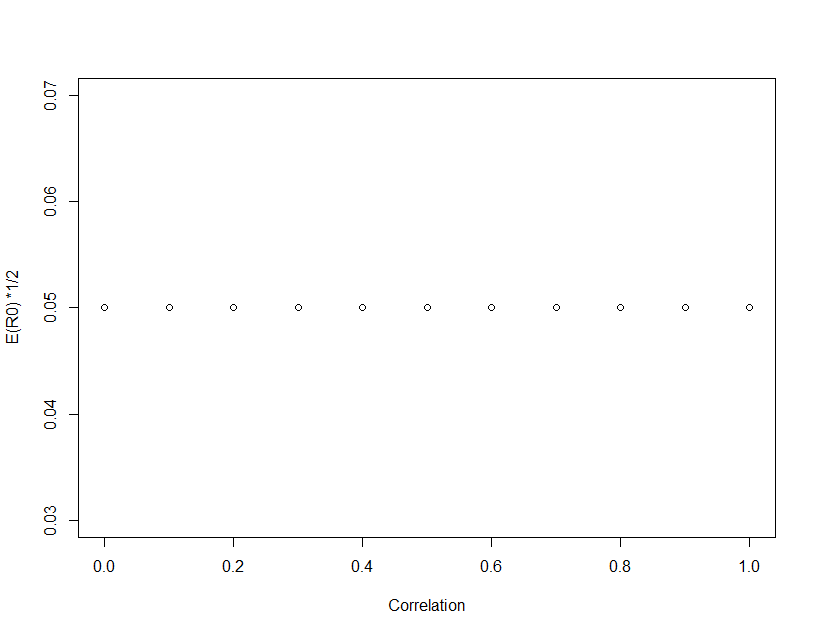
\includegraphics[scale=0.35]{exact_m=2}
	\caption{\footnotesize{Numerator of equation(\ref{eq1}) vs. correlation when m=2}}
	\label{fig1}
\end{figure}
\end{frame}

\begin{frame}[t]{Theoretical derivation}\vspace{10pt}

\begin{equation} \label{eq3}
\begin{split}
Var[R^0(\Gamma)] &= E[(R^0(\Gamma))^2] - (E[R^0(\Gamma)])^2 \\
&= p\{z_1 > 1.645 \ and \ z_2 \leq 1.645 \ or \ z_2 > 1.645 \ and \\ 
&z_1 \leq 1.645 \}  + p\{z_1 > 1.645 \ and \ z_2 > 1.645 \} \times 2^2 \\
&- (E[R^0(\Gamma)])^2
\end{split}
\end{equation}

\end{frame}


\begin{frame}[t]{Theoretical derivation}\vspace{10pt}
\begin{figure}[h]
	\centering
	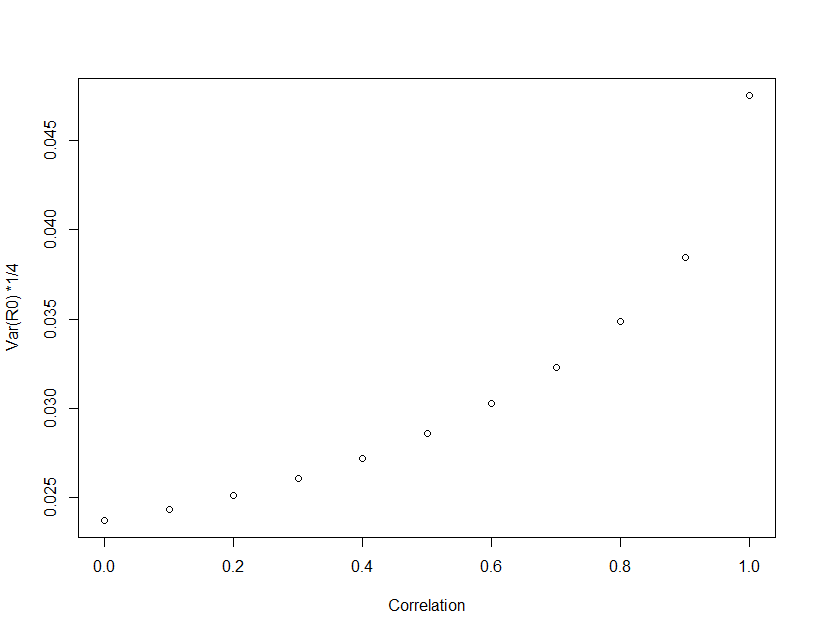
\includegraphics[scale=0.35]{exact_m=2_var}
	\caption{\footnotesize{Exact variance of $R^0(\Gamma) \times 1/4$ vs. correlation when m=2}}
	\label{fig2}
\end{figure}

\end{frame}

\begin{frame}[t]{Simulation}\vspace{10pt}
Set up: $z_1 \sim N(0,1), z_2 \sim N(0.5,1), \rho \in \{0,0.1,...,1\}, n=200, B=5000$
\begin{figure}[h]
	\centering
	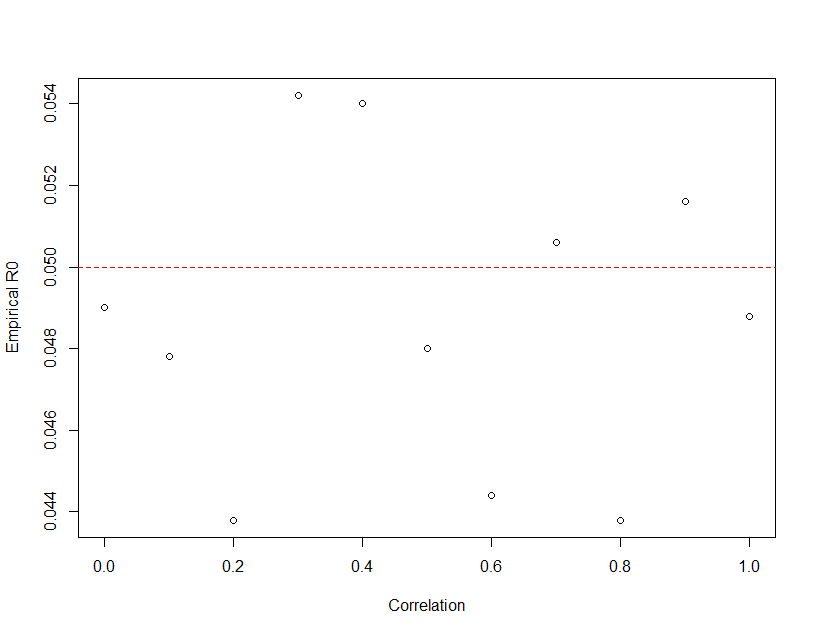
\includegraphics[scale=0.35]{empirical_m=2}
	\caption{\footnotesize{Mean of \# false rejections vs. correlation when m=2}}
	\label{fig3}
\end{figure}
\end{frame}

\begin{frame}[t]{Simulation}\vspace{10pt}
Empirical variance:
\begin{figure}[h]
	\centering
	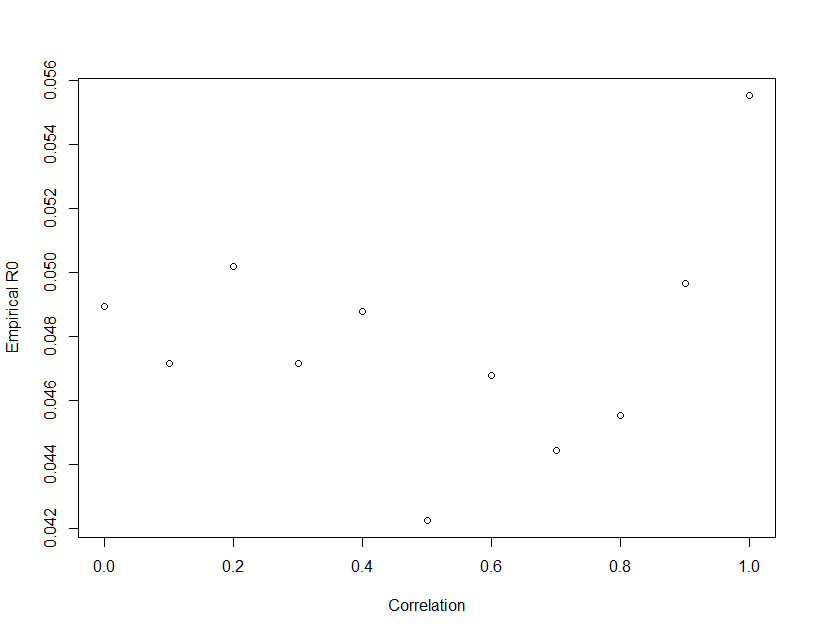
\includegraphics[scale=0.35]{empirical_m=2_var}
	\caption{\footnotesize{Variance of \# false rejections vs. correlation when m=2}}
	\label{fig4}
\end{figure}
\end{frame}


\begin{frame}[t]{M=3}\vspace{10pt}
Exact mean:
\begin{figure}[h]
	\centering
	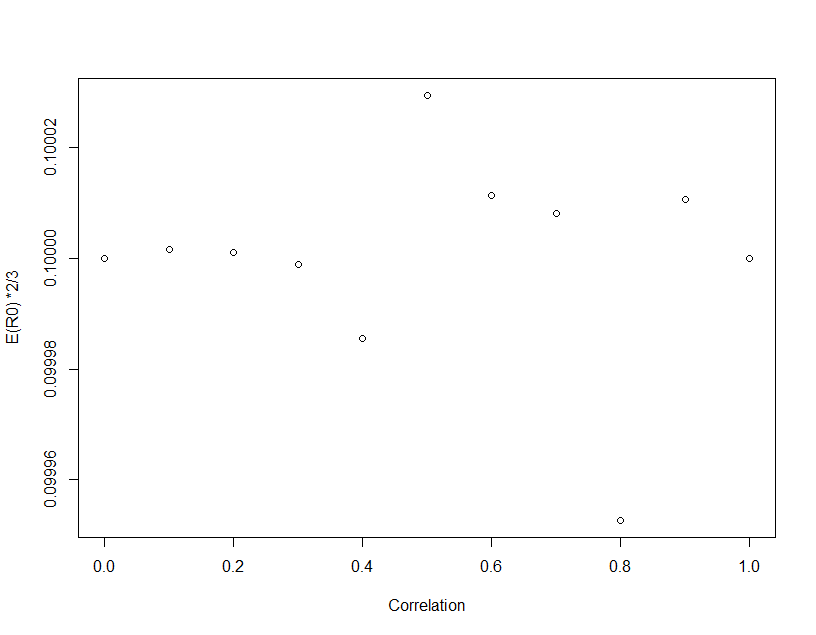
\includegraphics[scale=0.35]{exact_m=3}
	\caption{\footnotesize{Numerator of equation(\ref{eq1}) vs. correlation when m=3}}
	\label{fig5}
\end{figure}
\end{frame}

\begin{frame}[t]{M=3}\vspace{10pt}
Empirical mean:
\begin{figure}[h]
	\centering
	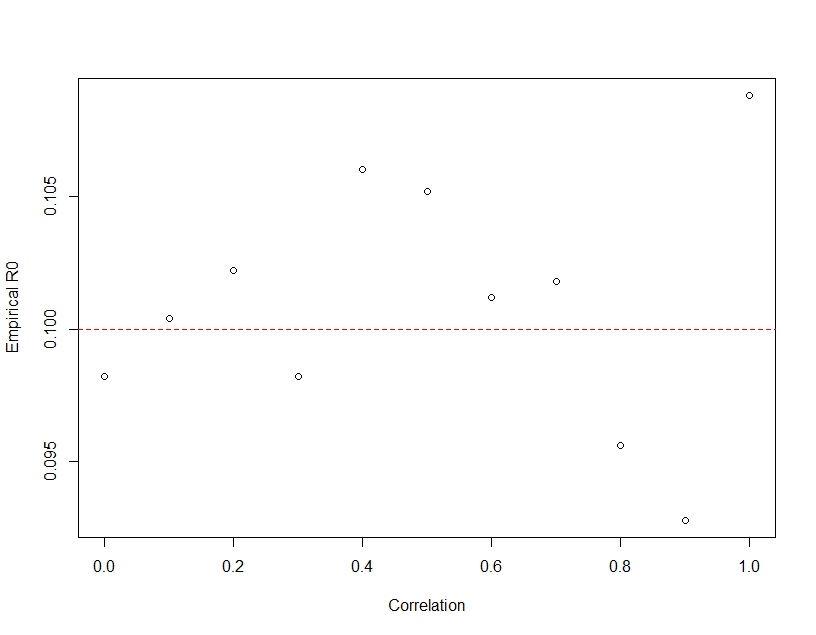
\includegraphics[scale=0.35]{empirical_m=3}
	\caption{\footnotesize{Mean of \# false rejections vs. correlation when m=3}}
	\label{fig6}
\end{figure}
\end{frame}

\begin{frame}[t]{M=3}\vspace{10pt}
Exact variance:
\begin{figure}[h]
	\centering
	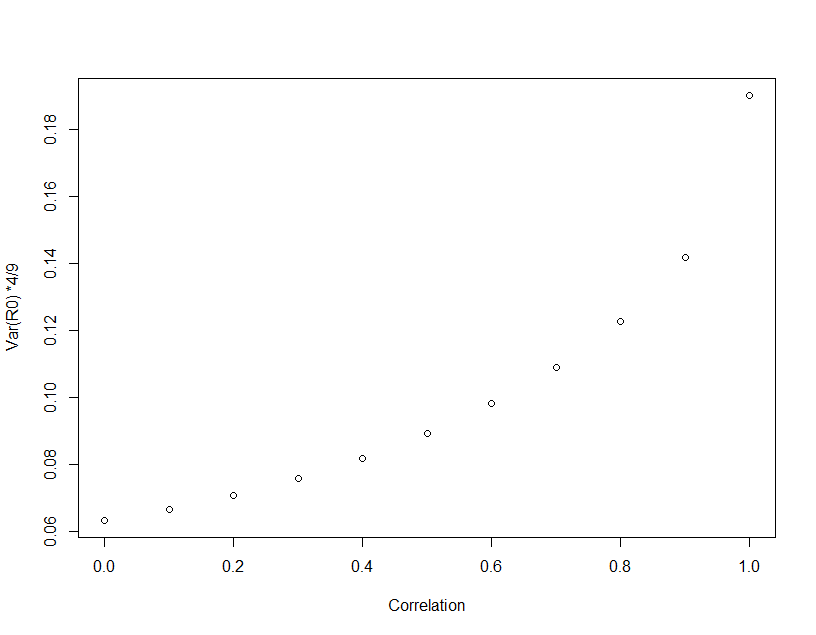
\includegraphics[scale=0.35]{exact_m=3_var}
	\caption{\footnotesize{Exact variance of $R^0(\Gamma) \times 1/4$ vs. correlation when m=3}}
	\label{fig7}
\end{figure}
\end{frame}


\begin{frame}[t]{M=3}\vspace{10pt}
Empirical variance:
\begin{figure}[h]
	\centering
	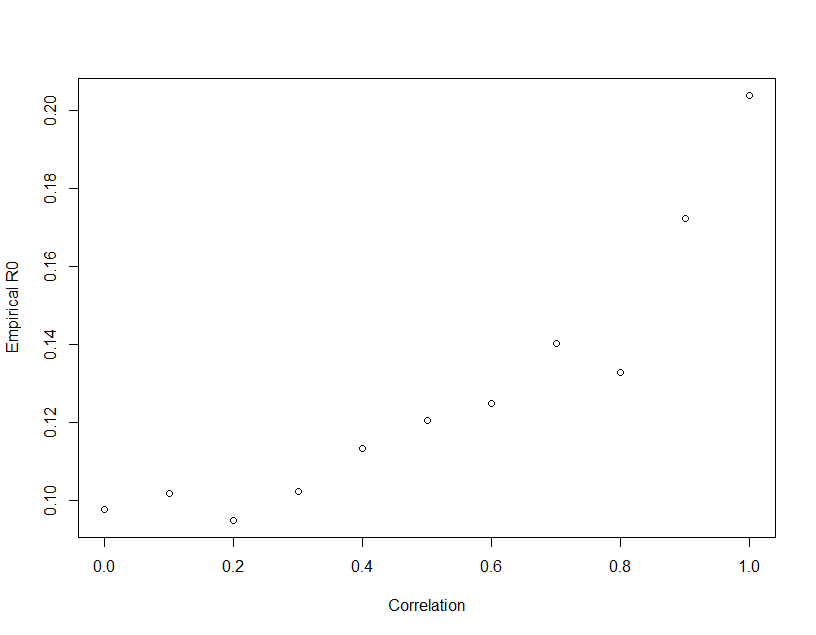
\includegraphics[scale=0.35]{empirical_m=3_var}
	\caption{\footnotesize{Variance of \# false rejections vs. correlation when m=3}}
	\label{fig8}
\end{figure}
\end{frame}

\begin{frame}[t]{Simulation when M=100}\vspace{10pt}
Set up: $z_i \sim N(\mu_i,1), \mu_i =0 \ for \ i \in \{1,2,...90\}, \mu_i = 0.5\ for \ i \in \{91,92,...,100\}$. They have equal correlations $\rho \in \{0,0.1,...,1\}$, $n=200$, $B=5000$.
\end{frame}

\begin{frame}[t]{Simulation when M=100}\vspace{10pt}
Empirical mean
\begin{figure}[h]
	\centering
	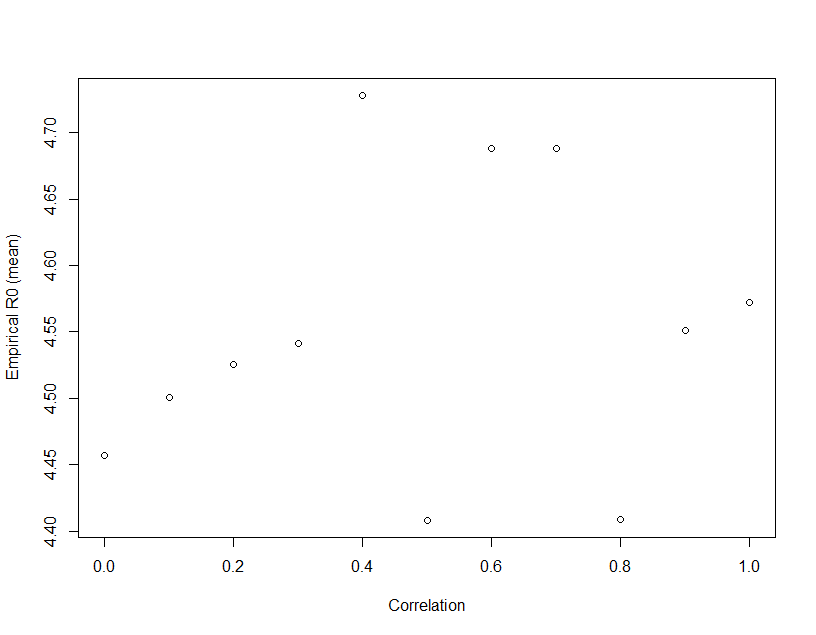
\includegraphics[scale=0.35]{empirical_m=100}
	\caption{\footnotesize{Mean of \# false rejections vs. correlation when m=100}}
	\label{fig9}
\end{figure}
\end{frame}



\begin{frame}[t]{Simulation when M=100}\vspace{10pt}
Empirical variance
\begin{figure}[h]
	\centering
	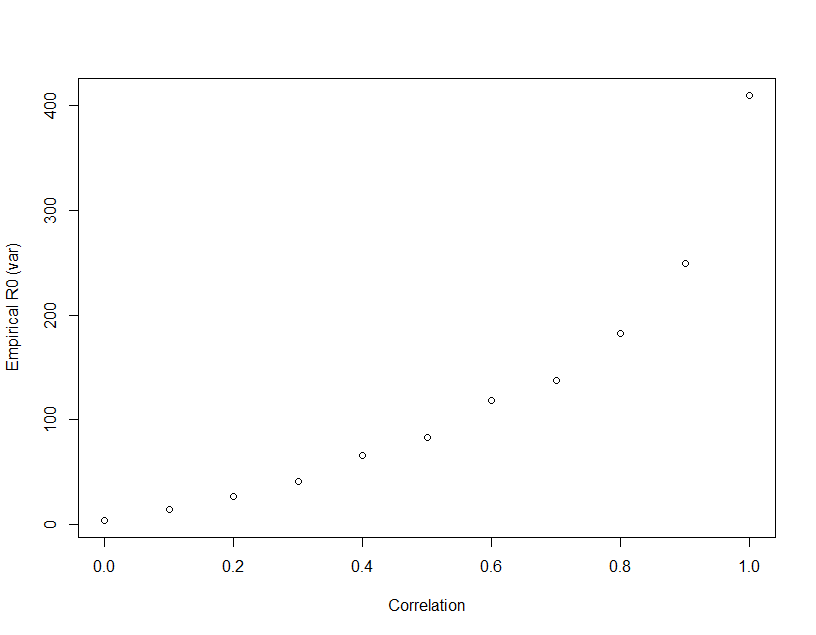
\includegraphics[scale=0.35]{empirical_m=100_var}
	\caption{\footnotesize{Variance of \# false rejections vs. correlation when m=100}}
	\label{fig9}
\end{figure}

\end{frame}


\end{document}